%%%%%%%%%%%%%%%%%%%%%%%%%%%%%%%%%%%%%%%%%%%%%%%%%%%%%%%%%%%%%%%%%%%%%%%%%%%%%%%
%
%  Chapter 5:  Three-Dimensional Leading-Edge Receptivity, Figures
%
%  S. Scott Collis
%
%  Written: 9-5-95
%
%  Revised: 1-3-97
%
%%%%%%%%%%%%%%%%%%%%%%%%%%%%%%%%%%%%%%%%%%%%%%%%%%%%%%%%%%%%%%%%%%%%%%%%%%%%%%%

%==============================================================================
%
%  Tables
%
%==============================================================================

%\begin{table}[p]
%\centering
%\begin{tabular}{|r||r|r|r|r|r|r|}
%\hline
%\multicolumn{1}{|c||}{Case} & 
%\multicolumn{1}{c|}{\M} & 
%\multicolumn{1}{c|}{\Re} & 
%\multicolumn{1}{c|}{\Pr} & 
%\multicolumn{1}{c|}{$\Lambda$} & 
%\multicolumn{1}{c|}{$n_\xi$} & 
%\multicolumn{1}{c|}{$n_\eta$} \\ \hline \hline
% B1 & 0.1 &    1 & 0.7 & $0^\circ$ & 256 &  63 \\ \hline
% B2 & 0.1 &   10 & 0.7 &  $0^\circ$ & 256 &  63 \\ \hline
% B3 & 0.1 &  100 & 0.7 &  $0^\circ$ & 256 &  63 \\ \hline
% B4 & 0.1 &  100 & 0.7 &  $0^\circ$ & 384 & 127 \\ \hline
% B5 & 0.1 & 1000 & 0.7 &  $0^\circ$ & 384 & 127 \\ \hline
% B6 & 0.5 & 1000 & 0.7 &  $0^\circ$ & 384 & 127 \\ \hline
% B7 & 0.7071 & 1414 & 0.7 & $45^\circ$ & 384 & 127 \\ \hline
% B8 & 0.7071 & 1414 & 0.7 & $45^\circ$ & 256 & 127 \\ \hline
% B9 & 0.8 &   10 & 0.7 &  $0^\circ$ & 256 &  63 \\ \hline
%B10 & 0.8 &   10 & 0.7 &  $0^\circ$ & 384 & 127 \\ \hline
%B11 & 0.8 &  100 & 0.7 &  $0^\circ$ & 256 &  63 \\ \hline
%B12 & 0.8 & 1000 & 0.7 &  $0^\circ$ & 384 & 127 \\ \hline
%\end{tabular}
%\caption {Parabolic cylinder base-flow parameters \label{t:mean}}
%\end{table}

%\begin{table}[p]
%\centering
%\begin{sideways}
%\begin{tabular}{|r||r|r|r|r|r|r|r|r|r|r|r|r|r|r|r|}
%\hline
%\multicolumn{1}{|c||}{Case} & 
%\multicolumn{1}{c|}{\M} & 
%\multicolumn{1}{c|}{\Re} & 
%\multicolumn{1}{c|}{\Pr} & 
%\multicolumn{1}{c|}{$T_w$} & 
%\multicolumn{1}{c|}{$\theta$} & 
%\multicolumn{1}{c|}{$x_{min}$} & 
%\multicolumn{1}{c|}{$x_{max}$} & 
%\multicolumn{1}{c|}{$n_\xi$} & 
%\multicolumn{1}{c|}{$n_\eta$} &
%\multicolumn{1}{c|}{$\Delta s_{min}$} &
%\multicolumn{1}{c|}{$b_s$} &
%\multicolumn{1}{c|}{$s_c$} &
%\multicolumn{1}{c|}{$\Delta n_{min}$} &
%\multicolumn{1}{c|}{$b_n$} &
%\multicolumn{1}{c|}{$n_c$} \\ \hline \hline
% 1 & 0.1 & 1000 & 0.7 & $T_{,n}=0$ & $0$ & -500 & 500 &
% 384 & 127 & 0.02 & 9 & 0.25 & $5\times 10^{-4}$ & 9 & 0.75 \\ \hline
% 2 & 0.8 & $1\times 10^5$ & 1.0 & $T_0$ & $35^\circ$ & -500 & 500 &
% 256 & 127 & 0.02 & 9 & 0.25 & $5\times 10^{-4}$ & 9 & 0.75 \\ \hline
%\end{tabular}
%\end{sideways}
%\caption {Swept base-flow parameters \label{t:swept}}
%\end{table}

\begin{table}[p]
\centering
\begin{tabular}{|r||r|r|r|r|r|r|r|r|r|}
\hline
\multicolumn{1}{|c||}{} & 
\multicolumn{1}{c|}{$\delta_1$} & 
\multicolumn{1}{c|}{$\delta_2$} & 
\multicolumn{1}{c|}{} &
\multicolumn{1}{c|}{} & 
\multicolumn{1}{c|}{$\theta_e$} &
\multicolumn{1}{c|}{} & 
\multicolumn{1}{c|}{} &
\multicolumn{1}{c|}{} &
\multicolumn{1}{c|}{} \\ 
\multicolumn{1}{|c||}{ \raisebox{1.5ex}[0cm][0cm]{$s$} } & 
\multicolumn{1}{c|}{$\times 100$} & 
\multicolumn{1}{c|}{$\times 100$} & 
\multicolumn{1}{c|}{ \raisebox{1.5ex}[0cm][0cm]{$U_e$} } &
\multicolumn{1}{c|}{ \raisebox{1.5ex}[0cm][0cm]{$T_e$} } & 
\multicolumn{1}{c|}{(deg.)} &
\multicolumn{1}{c|}{ \raisebox{1.5ex}[0cm][0cm]{$\frac{{w_s}_{max}}{U_e}$} } & 
\multicolumn{1}{c|}{ \raisebox{1.5ex}[0cm][0cm]{$\chi$} } & 
\multicolumn{1}{c|}{ \raisebox{1.5ex}[0cm][0cm]{$\M_e$} } &
\multicolumn{1}{c|}{ \raisebox{1.5ex}[0cm][0cm]{$\beta_h$} } \\ \hline \hline
0.020 & 0.324 & 0.119 & 0.700 & 1.128 & 88.7 & -0.006 & 7 & 0.527 & 1.000\\ \hline
0.041 & 0.324 & 0.119 & 0.700 & 1.128 & 87.3 & -0.012 & 14 & 0.527 & 0.999\\ \hline
0.085 & 0.324 & 0.120 & 0.703 & 1.128 & 84.5 & -0.024 & 28 & 0.529 & 0.996\\ \hline
0.109 & 0.325 & 0.120 & 0.705 & 1.127 & 82.9 & -0.031 & 36 & 0.531 & 0.993\\ \hline
0.136 & 0.325 & 0.120 & 0.708 & 1.127 & 81.2 & -0.038 & 45 & 0.533 & 0.989\\ \hline
0.197 & 0.326 & 0.121 & 0.717 & 1.125 & 77.5 & -0.053 & 63 & 0.540 & 0.978\\ \hline
0.233 & 0.328 & 0.122 & 0.723 & 1.124 & 75.4 & -0.061 & 73 & 0.545 & 0.970\\ \hline
0.273 & 0.329 & 0.123 & 0.731 & 1.122 & 73.2 & -0.069 & 84 & 0.552 & 0.960\\ \hline
0.368 & 0.334 & 0.125 & 0.752 & 1.118 & 68.5 & -0.084 & 105 & 0.569 & 0.931\\ \hline
0.423 & 0.338 & 0.127 & 0.766 & 1.116 & 66.0 & -0.090 & 116 & 0.580 & 0.912\\ \hline
0.485 & 0.344 & 0.129 & 0.781 & 1.113 & 63.6 & -0.096 & 126 & 0.592 & 0.890\\ \hline
0.553 & 0.351 & 0.132 & 0.799 & 1.109 & 61.1 & -0.101 & 136 & 0.607 & 0.864\\ \hline
0.712 & 0.371 & 0.140 & 0.838 & 1.101 & 56.5 & -0.106 & 153 & 0.639 & 0.801\\ \hline
0.802 & 0.384 & 0.144 & 0.860 & 1.096 & 54.5 & -0.107 & 161 & 0.657 & 0.765\\ \hline
0.904 & 0.400 & 0.150 & 0.881 & 1.091 & 52.5 & -0.106 & 168 & 0.675 & 0.727\\ \hline
1.014 & 0.419 & 0.156 & 0.903 & 1.086 & 50.8 & -0.105 & 174 & 0.693 & 0.688\\ \hline
2.091 & 0.618 & 0.221 & 1.030 & 1.055 & 42.8 & -0.087 & 208 & 0.803 & 0.425\\ \hline
4.098 & 0.953 & 0.326 & 1.111 & 1.033 & 39.0 & -0.066 & 232 & 0.874 & 0.241\\ \hline
6.167 & 1.239 & 0.415 & 1.143 & 1.024 & 37.7 & -0.055 & 242 & 0.904 & 0.168\\ \hline
8.210 & 1.483 & 0.491 & 1.159 & 1.019 & 37.1 & -0.048 & 248 & 0.919 & 0.131\\ \hline
10.013 & 1.676 & 0.550 & 1.169 & 1.016 & 36.8 & -0.043 & 251 & 0.928 & 0.110\\ \hline
15.479 & 2.175 & 0.705 & 1.185 & 1.011 & 36.2 & -0.034 & 255 & 0.943 & 0.075\\ \hline
20.261 & 2.544 & 0.818 & 1.192 & 1.009 & 35.9 & -0.030 & 256 & 0.949 & 0.060\\ \hline
25.164 & 2.879 & 0.922 & 1.197 & 1.007 & 35.8 & -0.027 & 255 & 0.954 & 0.049\\ \hline
30.121 & 3.185 & 1.016 & 1.200 & 1.006 & 35.7 & -0.024 & 254 & 0.957 & 0.042\\ \hline
40.092 & 3.733 & 1.186 & 1.204 & 1.005 & 35.5 & -0.021 & 251 & 0.961 & 0.033\\ \hline
50.083 & 4.216 & 1.335 & 1.207 & 1.004 & 35.4 & -0.018 & 249 & 0.964 & 0.027\\ \hline
\end{tabular}
\caption [Swept parabolic-cylinder boundary-layer characteristics] {Swept
parabolic-cylinder boundary-layer characteristics for $\M=0.8$,
$\Re=1\times10^{5}$, $\Pr=1$, and $T_w = T_0$.  Crossflow Reynolds number,
$\chi$, is defined in equation (\protect\ref{e:chi}) and the Hartree
parameter, $\beta_h$, is defined by equation
(\protect\ref{e:betah}). \label{t:results}}
\end{table}

\begin{table}[p]
\centering
\begin{tabular}{|r||r|r|r|r|r|r|r|}
\hline
\multicolumn{1}{|c||}{Case} & 
\multicolumn{1}{c|}{$s_w$} & 
\multicolumn{1}{c|}{$s_l$} & 
\multicolumn{1}{c|}{$A_l$} & 
\multicolumn{1}{c|}{$N_w$} & 
\multicolumn{1}{c|}{$N_l$} & 
\multicolumn{1}{c|}{$A_w$} & 
\multicolumn{1}{c|}{$A_{np}$} \\ \hline \hline
1 & 0.40 & 1.3997 & 4.0933 & 0.0709 & 2.3166 & 0.4333 & 0.4036 \\ \hline 
2 & 0.45 & 1.2014 & 3.2454 & 0.0043 & 1.7999 & 0.5388 & 0.5365 \\ \hline 
3 & 0.50 & 1.3997 & 6.2504 & 0.0097 & 2.3166 & 0.6224 & 0.6163 \\ \hline 
4 & 0.55 & 1.3997 & 6.4534 & 0.0611 & 2.3166 & 0.6764 & 0.6364 \\ \hline 
5 & 0.60 & 1.3997 & 6.2156 & 0.1457 & 2.3166 & 0.7090 & 0.6129 \\ \hline 
6 & 0.70 & 1.3997 & 5.0748 & 0.3754 & 2.3166 & 0.7284 & 0.5004 \\ \hline 
7 & 0.80 & 1.3997 & 3.7751 & 0.6475 & 2.3166 & 0.7113 & 0.3723 \\ \hline 
8 & 0.90 & 1.3997 & 2.6939 & 0.9369 & 2.3166 & 0.6779 & 0.2656 \\ \hline 
9 & 2.00 & 4.0036 & 1.3979 & 3.5579 & 4.9883 & 0.3344 & 0.0095 \\ \hline 
10 & 2.50 & 4.0036 & 0.5357 & 4.2538 & 4.9883 & 0.2570 & 0.0037 \\ \hline 
11 & 3.00 & 4.1999 & 0.2706 & 4.7009 & 4.9639 & 0.2080 & 0.0019 \\ \hline 
\end{tabular}
\caption[Crossflow receptivity results for $\beta=100$.] {Crossflow
receptivity results for $\beta=100$. Flow conditions are $\M=0.8$,
$\Re=1\times 10^5$, and $\theta=35^\circ$. \label{t:beta100} }
\end{table}

\begin{table}[p]
\centering
\begin{tabular}{|r||r|r|r|r|r|r|r|}
\hline
\multicolumn{1}{|c||}{Case} & 
\multicolumn{1}{c|}{$s_w$} & 
\multicolumn{1}{c|}{$s_l$} & 
\multicolumn{1}{c|}{$A_l$} & 
\multicolumn{1}{c|}{$N_w$} & 
\multicolumn{1}{c|}{$N_l$} & 
\multicolumn{1}{c|}{$A_w$} & 
\multicolumn{1}{c|}{$A_{np}$} \\ \hline \hline
1 & 0.30 & 2.0012 & 0.6041 & 0.1262 & 2.4554 & 0.0588 & 0.0518  \\ \hline
2 & 0.40 & 2.0012 & 2.4038 & 0.0001 & 2.4554 & 0.2063 & 0.2063  \\ \hline
3 & 0.50 & 2.0012 & 4.9201 & 0.0490 & 2.4554 & 0.4435 & 0.4223  \\ \hline
4 & 0.60 & 2.0012 & 6.8010 & 0.1528 & 2.4555 & 0.6800 & 0.5837  \\ \hline
5 & 0.70 & 2.0028 & 7.5289 & 0.2849 & 2.4579 & 0.8571 & 0.6446  \\ \hline
6 & 0.80 & 2.0012 & 7.3646 & 0.4354 & 2.4555 & 0.9769 & 0.6320  \\ \hline
7 & 1.00 & 2.5094 & 12.4113 & 0.7680 & 3.2134 & 1.0760 & 0.4992  \\ \hline
8 & 1.20 & 2.5094 & 8.6871 & 1.1172 & 3.2134 & 1.0679 & 0.3494  \\ \hline
9 & 1.50 & 2.5000 & 4.6284 & 1.6377 & 3.2000 & 0.9703 & 0.1887  \\ \hline
10 & 2.50 & 6.0009 & 27.6655 & 3.2000 & 7.0173 & 0.6083 & 0.0248  \\ \hline
11 & 4.00 & 7.0056 & 5.0805 & 5.1042 & 7.7820 & 0.3491 & 0.0021  \\ \hline
12 & 5.00 & 7.0056 & 1.3736 & 6.1357 & 7.7820 & 0.2648 & 0.0006  \\ \hline
13 & 7.00 & 12.0000 & 2.4094 & 7.7780 & 10.4235 & 0.1710 & 0.0001  \\ \hline
\end{tabular}
\caption[Crossflow receptivity results for $\beta=35$] {Crossflow receptivity
results for $\beta=35$. Flow conditions are $\M=0.8$, $\Re=1\times 10^5$, and
$\theta=35^\circ$. \label{t:beta35} }
\end{table}

\clearpage

%==============================================================================
%
%  Figures
%
%==============================================================================
%
%.... Parabolic-Cylinder Geometry
%
\begin{figure}[p]
\centering
\epsfxsize=4.25in \epsfboxo{figures/ch5/pcyl.ai}
%\includegraphics[width=4.25in]{figures/ch5/pcyl.ai}
\caption {Swept parabolic-cylinder geometry. \label{f:pcyl}}
\end{figure}
%
%.... Potential solution
%
\begin{figure}[p]
\centering
\figlab 3.3in 0in {$x$}
\figlab -0.1in 3.225in {$y$}
\epsfxsize=3.25in 
\epsfboxo{figures/ch3/pcyl-pot.ai}
%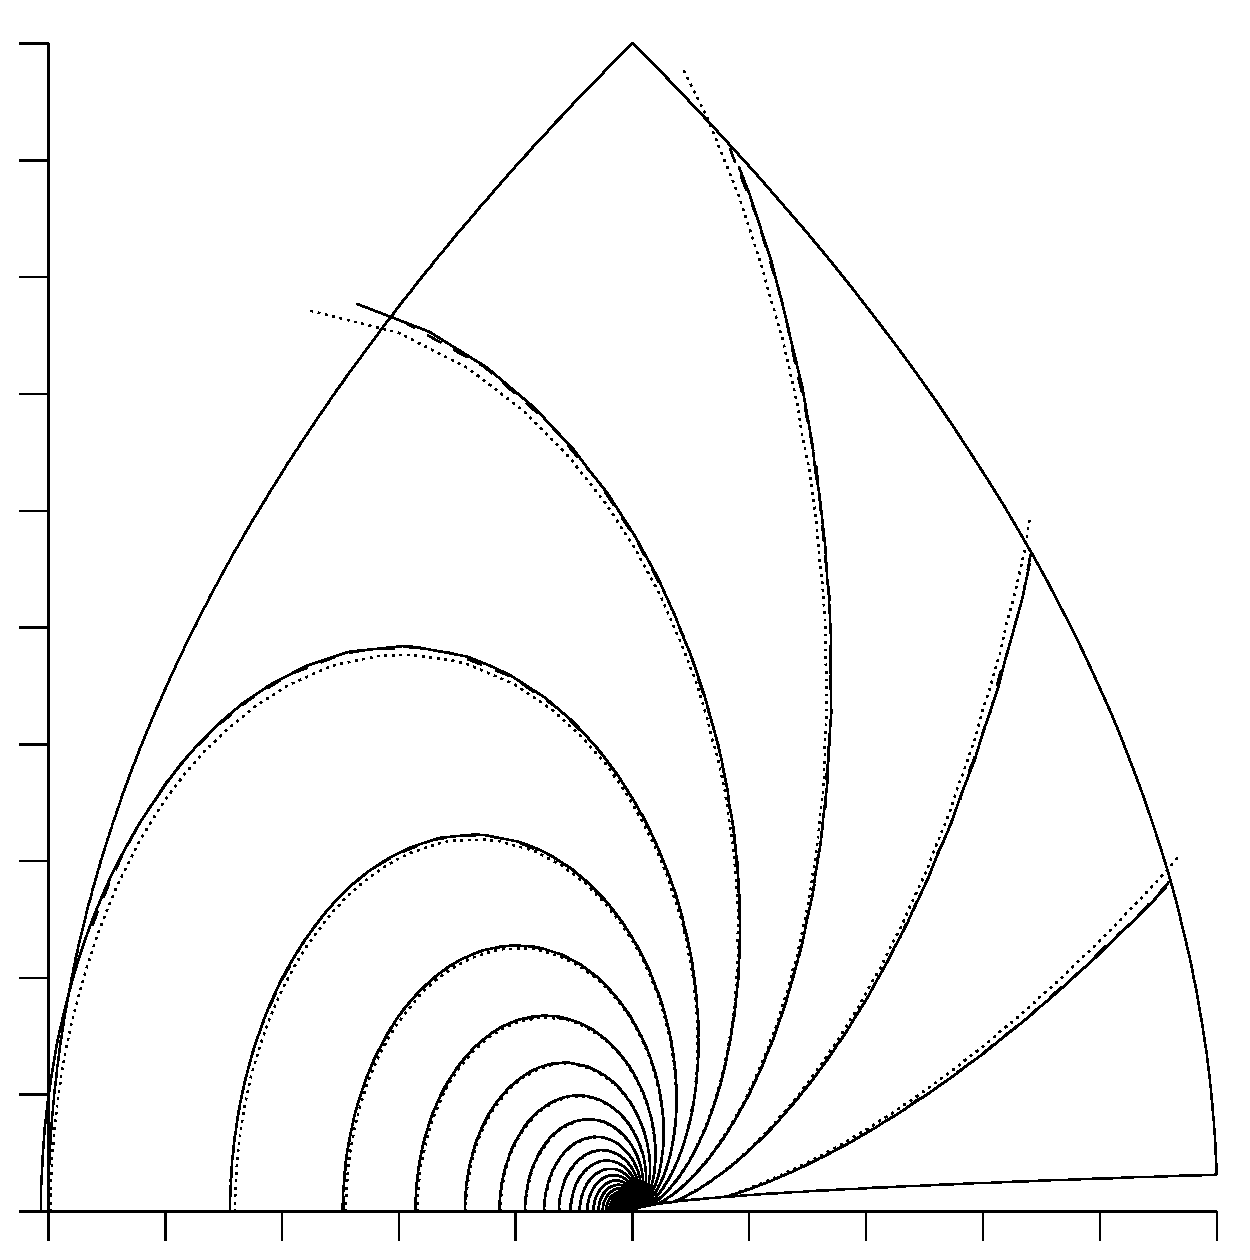
\includegraphics[width=3.25in]{figures/ch3/pcyl-pot.ai}
\caption [Contours of $C_p$ for $\M=0.8$, $\Re=1000$ flow over a parabolic
cylinder]{Contours of $C_p$ for $\M=0.8$, $\Re=1000$ flow over a parabolic
cylinder.  Results from three domain sizes are shown: \solid $x^*/r_n^* \in
\pm 1\times 10^8$, \dashed $\pm 1\times 10^7$, and \dotted $\pm 1\times 10^6$.
Contours are from 0 to 1.2 in increments of 0.02; tics every $100 r_n$.  Note
that $10^8$ and $10^7$ contours over-lie each other. \label{f:Cp-pot}}
\end{figure}
%
\begin{figure}[p]
\centering
\sethlabel{$s$}
\setvlabel{$\partial p/\partial s$}
\epsfxsize=5.25in 
\epsfboxo{figures/ch3/pcyl-pgrad.eps}
\caption [Pressure gradient along the wall for two domain sizes]{Pressure
gradient along the wall for two domain sizes: \solid $x^*/r_n^* \in \pm
1\times 10^8$ and \dashed $\pm 1\times 10^7$. \label{f:pg-pot}}
\end{figure}
%
\begin{figure}[p]
\centering
\figlab 3.3in 0in {$x$}
\figlab -0.1in 3.225in {$y$}
\epsfxsize=3.25in 
\epsfboxo{figures/ch3/pcyl-int.ai}
\caption [Contours of $C_p$ from the potential solution at $\M=0.8$, $\Re=1000$
after interpolation to a Navier--Stokes mesh]{Contours of $C_p$ from the
potential solution at $\M=0.8$, $\Re=1000$ after interpolation to a
Navier--Stokes mesh.  The \solid lines are the $x^*/r_n^* \in \pm 1\times
10^8$ potential solution while the \dashed lines are the interpolated
solution.  Note that they are very nearly identical.  Contours are from 0 to
1.2 in increments of 0.02; tics every $100 r_n$.  \label{f:Cp-interp}}
\end{figure}
%
%.... Mesh generation
%
\begin{figure}[p]
\centering
\figlab 3.3in 0in {$x$}
\figlab -0.1in 3.225in {$y$}
\epsfxsize=3.25in 
\epsfboxo{figures/ch5/grid.eps}
\caption[Typical Parabolic cylinder mesh] {Typical Parabolic cylinder mesh:
$x_{min} = -500$, $x_{max}=500$.  Tic marks are at every $100 r_n$.  (This
particular mesh uses the same distribution but with fewer points than that
used in the $\Re=1000$ calculations.)
\label{f:pcylmesh}}
\end{figure}
%
\begin{figure}[p]
\centering
\setvlabel{$\tilde\xi$}
\epsfxsize=4in 
\epsfboxo{figures/ch5/f40.eps}
\setvlabel{$\tilde\xi_{,\xi}$}
\epsfxsize=4in 
\epsfboxo{figures/ch5/f41.eps}
\sethlabel{$\xi$}
\setvlabel{$\tilde\xi_{,\xi\xi}$}
\epsfxsize=4in 
\epsfboxo{figures/ch5/f42.eps}
\caption [Mapping function and its derivatives for parameters typical of those
used in the wall-tangent direction]{Mapping function and its derivatives for
parameters typical of those used in the wall-tangent direction:
$\Delta\tilde\xi_{min}=0.001$, $N_\xi = 768$, $\tilde\xi_{max}=25$,
$\xi_c=0.25$, $b=7$.
\label{f:map}}
\end{figure}
%
%\begin{figure}[p]
%\centering
%\nofig{5in}{3in}
%\caption {Comparison of mapping functions \label{f:mapcomp}}
%\end{figure}
%
%\begin{figure}[p]
%\centering
%\nofig{5in}{3in} % \epsfxsize=4.0in \epsfboxo{figures/}
%\caption {Near wall pressure with both mapping functions. \label{f:mappres}}
%\end{figure}
%
%.... $\M=0.1$, $\Re=1000$, $\Lambda=0$ mean flow results
%
\begin{figure}[p]
\centering
\sethlabel{$N_{\rm step}$}
\setvlabel{$||{\rm Residual}||$}
\epsfxsize=5.4in 
\epsfboxo{figures/ch5/M=0.1_long_conv.eps}
\caption {Convergence history for $\M=0.1$, $\Re=1000$ mean flow calculation.
\label{f:conv}}
\end{figure}
%
%.... comparison with Davis' results
%
\begin{figure}[p]
\centering
\setvlabel{$\omega_D$}
\sethlabel{$\xi_D$}
\epsfxsize=5.4in 
%\epsfboxo{figures/ch5/davis.eps}
\epsfboxo{figures/ch5/f56.eps}
\caption [Vorticity along the surface of the parabolic cylinder plotted in the
coordinates of Davis \protect\cite{Davis:72}.]{Vorticity along the surface of
the parabolic cylinder plotted in the coordinates of Davis
\protect\cite{Davis:72}.  Lines denote the current solution at $\M=0.1$ while
symbols are taken from Davis' incompressible solutions: \solid, \scircle are
at $\Re=100$ and \dotted, $\times$ are at $\Re=1000$. \label{f:davis}}
\end{figure}
%
\clearpage
%
%.... comparison with incompressible parabolized results
%
\begin{figure}[p]
\centering
\sethlabel{$\xi_D$}
\setvlabel{$\omega_D$}
\epsfxsize=5.4in \epsfboxo{figures/ch5/machvort.eps}
\caption [Effect of compressibility on the scaled wall-vorticity]{Effect of
compressibility on the scaled wall-vorticity at $\Re=1000$, $\Pr = 0.7$:
\scircle incompressible, \solid $\M=0.1$, \dashed $\M=0.5$, and \dotted
$\M=0.8$
\label{f:mach} }
\end{figure}
%
\begin{figure}[p]
\centering
\sethlabel{$\M^2$}
\setvlabel{$\omega_D(0)$}
\epsfxsize=5.4in \epsfboxo{figures/ch5/mach2vort.eps}
\caption [Variation of the scaled wall-vorticity at the attachment line with
the Mach number squared]{Variation of the scaled wall-vorticity at the
attachment line with the Mach number squared: $\Re=1000$,
$\Pr=0.7$. \label{f:attach} }
\end{figure}
%
\begin{figure}[p]
\centering
\sethlabel{$\xi_D$}
\setvlabel{$\omega_D$}
\epsfxsize=5.4in \epsfboxo{figures/ch5/vortpar.eps}
\caption [Comparison of wall vorticity with an incompressible parabolized
solution] {Comparison of wall vorticity with incompressible parabolized
solution, $\Re=1000$, $\Pr=0.7$: \solid $\M=0.1$ and \dashed $\M=0$
parabolized. \label{f:parabolic} }
\end{figure}
%
\begin{figure}[p]
\centering
\sethlabel{$s$}
\setvlabel{$\partial p / \partial s$}
\epsfxsize=5.4in \epsfboxo{figures/ch5/f57.eps}
\caption [Effect of Mach number on the pressure gradient at the wall.] {Effect
of Mach number on the pressure gradient, $\partial p/\partial s$, at the wall
for $\Re=1000$, $\Pr=0.7$: \solid $\M=0.1$, \dashed $\M=0.5$, \dotted
$\M=0.8$. \label{f:pg_mach} }
\end{figure}
%
%.... Swept parabolic cylinder mean flow
%
% \begin{figure}[p]
% \centering
% \nofig{5in}{3in}
% \caption {Example of a body-fitted mesh for boundary-layer analysis.
% \label{f:bfmesh}}
% \end{figure}
%
\begin{figure}[p]
\centering
\epsfxsize=5in \epsfbox{figures/ch5/3dbl_schematic.ai}
\caption [Schematic of a three-dimensional boundary layer]{Schematic of a
three-dimensional boundary layer near a swept leading-edge. Surface curvature
is not explicitly shown in order to simplify the presentation. \label{f:3dbl}
}
\end{figure}
%
\begin{figure}[p]
\centering
\sethlabel{$n$}
\setvlabel{$u_s/U_e$, $w_s/U_e$}
\epsfxsize=5.4in \epsfboxo{figures/ch5/f10.eps}
\caption [Velocity profiles at $s=0.197$] {Velocity profiles at $s=0.197$ in
local streamwise coordinates: \solid $u_s/U_e$, \dashed $w_s/U_e$.  Flow
conditions are $\M=0.8$, $\Re=1\times 10^5$, $\theta=35^\circ$.
\label{f:pro1} }
\end{figure}
%
\begin{figure}[p]
\centering
\sethlabel{$n$}
\setvlabel{$u_s/U_e$, $w_s/U_e$}
\epsfxsize=5.4in \epsfboxo{figures/ch5/f11.eps}
\caption [Velocity profiles at $s=0.802$] {Velocity profiles at $s=0.802$ in
local streamwise coordinates: \solid $u_s/U_e$, \dashed $w_s/U_e$.  Flow
conditions are $\M=0.8$, $\Re=1\times 10^5$, $\theta=35^\circ$. \label{f:pro2}
}
\end{figure}
%
\begin{figure}[p]
\centering
\sethlabel{$n$}
\setvlabel{$u_s/U_e$, $w_s/U_e$}
\epsfxsize=5.4in \epsfboxo{figures/ch5/f12.eps}
\caption [Velocity profiles at $s=2.09$] {Velocity profiles at $s=2.09$ in
local streamwise coordinates: \solid $u_s/U_e$, \dashed $w_s/U_e$.  Flow
conditions are $\M=0.8$, $\Re=1\times 10^5$, $\theta=35^\circ$. \label{f:pro3}
}
\end{figure}
%
\begin{figure}[p]
\centering
\sethlabel{$s$}
\setvlabel{${w_s}_{max} / U_e$}
\epsfxsize=5.4in \epsfboxo{figures/ch5/f5.eps}
\caption [Maximum, in the transverse direction, of the crossflow component of
\protect \\velocity] {Maximum, in the transverse direction, of the crossflow
component of velocity normalized by the local edge velocity for the flow
conditions: $\M=0.8$, $\Re=1\times 10^5$, $\theta=35^\circ$. \label{f:r4.wmax}
}
\end{figure}
%
\begin{figure}[p]
\centering
\sethlabel{$s$}
\setvlabel{$\theta_e$ (deg.)}
\epsfxsize=5.4in \epsfboxo{figures/ch5/f6.eps}
\caption[Evolution of the local sweep angle] {Evolution of the local sweep
angle for the conditions $\M=0.8$, $\Re=1\times 10^5$, $\theta=35^\circ$.
\label{f:r4.thetae} }
\end{figure}
%
\begin{figure}[p]
\centering
\sethlabel{$s$}
\setvlabel{$\beta_h$}
\epsfxsize=5.4in \epsfboxo{figures/ch5/f7.eps}
\caption[Evolution of the Hartree parameter] {Evolution of the Hartree
parameter for the flow conditions: $\M=0.8$, $\Re=1\times 10^5$,
$\theta=35^\circ$.
\label{f:r4.betah} }
\end{figure}
%
\begin{figure}[p]
\centering
\sethlabel{$s$}
\setvlabel{$\delta_1$, $\delta_2$}
\epsfxsize=5.4in \epsfboxo{figures/ch5/f8.eps}
\caption[Boundary layer displacement thickness and momentum thickness]
{Boundary layer displacement thickness and momentum thickness: \solid is the
displacement thickness, \dashed denotes the momentum thickness.  The flow
conditions are $\M=0.8$, $\Re=1\times 10^5$, $\theta=35^\circ$.
\label{f:r4.thick} }
\end{figure}
%
\begin{figure}[p]
\centering
\sethlabel{$s$}
\setvlabel{$H$}
\epsfxsize=5.4in \epsfboxo{figures/ch5/f9.eps}
\caption[Boundary layer shape factor] {Boundary layer shape factor for the
conditions: $\M=0.8$, $\Re=1\times 10^5$, $\theta=35^\circ$.
\label{f:r4.shape} }
\end{figure}
%
\clearpage
%
%.... Linear stability analysis
%
\begin{figure}[p]
\centering
\sethlabel{$n$}
\epsfxsize=5.4in \epsfboxo{figures/ch5/f13.eps}
\caption[Boundary layer profiles at the point of maximum crossflow] {Boundary
layer profiles at the point of maximum crossflow: \solid $\rho$, \dashed
$\vs$, \dotted $\vn$, \chndash $w$, and \chndot\  $T$. Conditions: $s=0.802$,
$\M=0.8$, $\Re=1\times 10^5$, $\theta=35^\circ$. \label{f:profile} }
\end{figure}
%
\begin{figure}[p]
\centering
\sethlabel{$\beta$}
\setvlabel{$\sigma$}
\epsfxsize=5.4in \epsfboxo{figures/ch5/f1.eps}
\caption[Quasi-parallel LST spatial growth-rate] {Quasi-parallel LST spatial
growth-rate: $s=0.802$, $\beta=35$, $\M=0.8$, $\Re=1\times 10^5$,
$\theta=35^\circ$. \label{f:sigma} }
\end{figure}
%
\begin{figure}[p]
\centering
\sethlabel{$\beta$}
\setvlabel{$\alpha$}
\epsfxsize=5.4in \epsfboxo{figures/ch5/f14.eps}
\caption[Quasi-parallel LST chordwise wavenumber] {Quasi-parallel LST
chordwise wavenumber: $s=0.802$, $\beta=35$, $\M=0.8$, $\Re=1\times 10^5$,
$\theta=35^\circ$. \label{f:alpha} }
\end{figure}
%
\begin{figure}[p]
\centering
\sethlabel{$\beta$}
\setvlabel{$\psi$ (deg.)}
\epsfxsize=5.4in \epsfboxo{figures/ch5/f15.eps}
\caption[Wave-angle variation predicted from quasi-parallel LST] {Wave-angle
variation predicted from quasi-parallel LST: $s=0.802$, $\beta=35$, $\M=0.8$,
$\Re=1\times 10^5$, $\theta=35^\circ$. \label{f:psi} }
\end{figure}
%
\begin{figure}[p]
\centering
\sethlabel{$s$}
\setvlabel{$\sigma$}
\epsfxsize=5.4in \epsfboxo{figures/ch5/f16.eps}
\caption[Quasi-parallel growth-rate without curvature] {Quasi-parallel
growth-rate without curvature for $\beta=35$, $\M=0.8$, $\Re=1\times 10^5$,
$\theta=35^\circ$. \label{f:QPNCsigma} }
\end{figure}
%
%\begin{figure}[p]
%\centering
%\sethlabel{$s$}
%\setvlabel{$\alpha$}
%\epsfxsize=5.4in \epsfboxo{figures/ch5/f17.eps}
%\caption [Quasi-parallel chordwise wavenumber without curvature]
%{Quasi-parallel chordwise wavenumber without curvature for $\beta=35$,
%$\M=0.8$, $\Re=1\times 10^5$, $\theta=35^\circ$. \label{f:QPNCalpha} }
%\end{figure}
%
\begin{figure}[p]
\centering
\sethlabel{$s$}
\setvlabel{$\sigma$}
\epsfxsize=5.4in \epsfboxo{figures/ch5/f18.eps}
\caption[Comparison of QPNC and LNS growth-rates] {Comparison of growth-rate
from QPNC \solid and LNS \dashed: $\beta=35$, $\M=0.8$, $\Re=1\times 10^5$,
$\theta=35^\circ$. \label{f:x5gr} }
\end{figure}
%
\begin{figure}[p]
\centering
\sethlabel{$s$}
\setvlabel{$\sigma$}
\epsfxsize=5.4in \epsfboxo{figures/ch5/f23.eps}
\caption[Comparison of QPNC, QPWC, and LNS growth-rates] {Comparison of
growth-rate from QPNC \solid, LNS \dashed, and \dotted QPWC: $\beta=35$,
$\M=0.8$, $\Re=1\times 10^5$, $\theta=35^\circ$. \label{f:QPWC} }
\end{figure}
%
\begin{figure}[p]
\centering
\sethlabel{$s$}
\setvlabel{$K \delta_1$}
\epsfxsize=5.4in \epsfboxo{figures/ch5/f22.eps}
\caption[Normalized surface curvature] {Normalized surface curvature for
$\M=0.8$, $\Re=1\times 10^5$, $\theta=35^\circ$. \label{f:radius} }
\end{figure}
%
\begin{figure}[p]
\centering
\sethlabel{$s$}
\setvlabel{$\sigma$}
\epsfxsize=5.4in \epsfboxo{figures/ch5/f19.eps}
\caption[Comparison of growth-rate predictions for NPWC and LNS] {Comparison
of growth-rate predictions: \solid QPNC, \dashed LNS, \dotted QPWC, \chndash\
NPWC.  Flow parameters: $\beta=35$, $\M=0.8$, $\Re=1\times 10^5$,
$\theta=35^\circ$. Note that LNS and NPWC curves overlap.  \label{f:NPWC} }
\end{figure}
%
\begin{figure}[p]
\centering
\figlab 1.0in 2.6in {\a}
\sethlabel{$s$}
\setvlabel{$\sigma$}
\epsfxsize=5.4in \epsfboxo{figures/ch5/f20.eps}
\vskip 0.5in
\figlab 1.0in 2.6in {\b}
\sethlabel{$s$}
\setvlabel{$\sigma$}
\epsfxsize=5.4in \epsfboxo{figures/ch5/f21.eps}
\caption[Terms contributing to the nonparallel growth-rate] {Terms
contributing to the nonparallel growth-rate: \solid QPWC, \dashed NPWC,
\dotted nonparallel meanflow, \chndash\ eigenfunction distortion.  Frame $(a)$
shows the entire unstable region, $(b)$ is a closeup near the leading-edge.
Flow parameters: $\beta=35$, $\M=0.8$, $\Re=1\times 10^5$, $\theta=35^\circ$.
\label{f:NPterms} }
\end{figure}
%
\begin{figure}[p]
\centering
\sethlabel{$s$}
\setvlabel{$\alpha$}
\epsfxsize=5.4in \epsfboxo{figures/ch5/f24.eps}
\caption[Comparison of QPNC, QPWC, and NPWC wavenumber predictions]
{Comparison of wavenumber predictions: \solid QPNC, \dashed QPWC, \dotted
NPWC.  Flow parameters: $\beta=35$, $\M=0.8$, $\Re=1\times 10^5$,
$\theta=35^\circ$. \label{f:NPwavenumber} }
\end{figure}
%
\begin{figure}[p]
\centering
\sethlabel{$s$}
\setvlabel{$\alpha$}
\epsfxsize=5.4in \epsfboxo{figures/ch5/f25.eps}
\caption[Comparison of QPWC, NPWC, and LNS wavenumber predictions] {Comparison
of wavenumber predictions: \solid QPWC, \dashed NPWC, \dotted LNS.  Flow
parameters: $\beta=35$, $\M=0.8$, $\Re=1\times 10^5$,
$\theta=35^\circ$. \label{f:NPwaveLNS} }
\end{figure}
%
\begin{figure}[p]
\centering
\sethlabel{$s$}
\setvlabel{$\sigma$}
\epsfxsize=5.4in \epsfboxo{figures/ch5/f26.eps}
\caption[Comparison of NPWC and LNS growth-rates near the leading-edge]
{Comparison of NPWC and LNS growth-rates near the leading-edge: \solid LNS,
\dashed NPWC.  Flow parameters: $\beta=35$, $\M=0.8$, $\Re=1\times 10^5$,
$\theta=35^\circ$. \label{f:LNSle} }
\end{figure}
%
\begin{figure}[p]
\centering
\sethlabel{$s$}
\setvlabel{$\sigma$}
\epsfxsize=5.4in \epsfboxo{figures/ch5/f29.eps}
\caption[Comparison of LNS and NPWC growth-rates] {Comparison of \solid LNS
and \dashed NPWC growth-rates for $\beta=100$, $\M=0.8$, $\Re=1\times 10^5$,
and $\theta=35^\circ$. \label{f:Beta100} }
\end{figure}
%
\clearpage
%
\begin{figure}[p]
\centering
\sethlabel{$s$}
\setvlabel{$\sigma$}
\epsfxsize=5.4in \epsfboxo{figures/ch5/f28.eps}
\caption[Contributions to nonparallel growth-rate for $\beta=100$]
{Contributions to nonparallel growth-rate: \solid QPWC, \dashed NPWC, \dotted
nonparallel meanflow term, and \chndash\ eigenfunction distortion term for
$\beta=100$, $\M=0.8$, $\Re=1\times 10^5$, and
$\theta=35^\circ$. \label{f:Beta100NPterms} }
\end{figure}
%
\begin{figure}[p]
\centering
\sethlabel{$s$}
\setvlabel{$\sigma$}
\epsfxsize=5.4in \epsfboxo{figures/ch5/f44.eps}
\caption[Growth-rate from multidomain approach for $\beta=100$] {Growth-rate
from two overlapping domains for $\beta=100$: \solid is domain for $s \in
[0.32,3.18]$ while \dashed is for $s \in [1.78,5.12]$.  The flow conditions
are $\M=0.8$, $\Re=1\times 10^5$, and $\theta=35^\circ$. \label{f:multidomain}
}
\end{figure}
%
%.... Full LNS growth-rate
%
\begin{figure}[p]
\centering
\figlab 3.75in 2.6in {\a $\beta = 35$}
\sethlabel{$s$}
\setvlabel{$\sigma$}
\epsfxsize=5.4in \epsfboxo{figures/ch5/f63.eps}
\vskip 0.5in
\figlab 3.75in 2.6in {\b $\beta = 100$}
\sethlabel{$s$}
\setvlabel{$\sigma$}
\epsfxsize=5.4in \epsfboxo{figures/ch5/f65.eps}
\caption[LNS growth-rate for $\beta=35$ and $\beta=100$ compared to NPWC] {LNS
growth-rate, based on $E'_k$, for \a $\beta=35$ and \b $\beta=100$ compared to
NPWC: \solid is LNS while \dashed is NPWC.  The flow conditions are $\M=0.8$,
$\Re=1\times 10^5$, and $\theta=35^\circ$. \label{f:63} }
\end{figure}
%
%.... Full LNS wavenumber
%
\begin{figure}[p]
\centering
\figlab 1.0in 2.6in {\a $\beta = 35$}
\sethlabel{$s$}
\setvlabel{$\alpha$}
\epsfxsize=5.4in \epsfboxo{figures/ch5/f62.eps}
\vskip 0.5in
\figlab 1.0in 2.6in {\b $\beta = 100$}
\sethlabel{$s$}
\setvlabel{$\alpha$}
\epsfxsize=5.4in \epsfboxo{figures/ch5/f64.eps}
\caption[LNS wavenumber for $\beta=35$ and $\beta=100$ compared to NPWC] {LNS
wavenumber, based on $|\hat\vs|_{max}$, for \a $\beta=35$ and \b $\beta=100$
compared to NPWC: \solid is LNS while \dashed is NPWC.  The flow conditions
are $\M=0.8$, $\Re=1\times 10^5$, and $\theta=35^\circ$. \label{f:62} }
\end{figure}
%
%.... N-factor plots
%
\begin{figure}[p]
\centering
\sethlabel{$s$}
\setvlabel{$N$-factor}
\epsfxsize=5.4in \epsfboxo{figures/ch5/f32.eps}
\caption[Evolution of the $N$-factor for $\beta=35$ and $\beta=100$]
{Evolution of the $N$-factor for \solid $\beta=35$ and \dashed $\beta=100$
with the flow conditions $\M=0.8$, $\Re=1\times 10^5$, and $\theta=35^\circ$.
\label{f:N-factor} }
\end{figure}
%
\begin{figure}[p]
\centering
\sethlabel{$s$}
\setvlabel{$N$-factor}
\epsfxsize=5.4in \epsfboxo{figures/ch5/f53.eps}
\caption[Comparison of the LNS and NPWC $N$-factors for $\beta=35$]
{Comparison of the $N$-factor for $\beta=35$: \solid is LNS and \dashed is
NPWC. The flow conditions are $\M=0.8$, $\Re=1\times 10^5$, and
$\theta=35^\circ$.
\label{f:N-35-factor} }
\end{figure}
%
\begin{figure}[p]
\centering
\sethlabel{$s$}
\setvlabel{$N$-factor}
\epsfxsize=5.4in \epsfboxo{figures/ch5/f54.eps}
\caption[Comparison of the LNS and NPWC $N$-factors for $\beta=100$]
{Comparison of the $N$-factor for $\beta=100$: \solid is LNS and \dashed is
NPWC. The flow conditions are $\M=0.8$, $\Re=1\times 10^5$, and
$\theta=35^\circ$.
\label{f:N-100-factor} }
\end{figure}
%
%.... Criteron for breakdown of nonparallel stability analysis
%
\begin{figure}[p]
\centering
\sethlabel{$s$}
\setvlabel{$\delta_g = \frac{\lambda_s}{\delta_1}
\left(\frac{\partial\delta_1}{\partial s}\right)$}
\epsfxsize=5.4in \epsfboxo{figures/ch5/NPmeasure.ai}
\caption[Approximate criterion for the failure of nonparallel LST]
{Approximate criterion for the failure of nonparallel linear stability theory:
\solid $\beta=35$, \dashed $\beta=100$. \label{f:NPmeasure} }
\end{figure}
%
%.... Finite Reynolds number results for FSC profile
%
\begin{figure}[p]
\centering
\sethlabel{$x$}
\setvlabel{${E'_k}^{1/2}$}
\epsfxsize=5.4in \epsfboxo{figures/ch5/f33.eps}
\caption[Evolution of ${E'_k}^{1/2}$ on a flat plate with parallel FSC
profile] {Evolution of ${E'_k}^{1/2}$ on a flat plate with parallel FSC
profile downstream of a bump at $x_w=0.7$ with $\sigma_w=0.05$: \solid LNS and
\dashed FRNT for the flow conditions $\beta=35$, $\M_e=0.657$, $\Re=1\times
10^5$, and $\theta_e=54.5^\circ$.
\label{f:FSC-35} }
\end{figure}
%
\begin{figure}[p]
\centering
\sethlabel{$x$}
\setvlabel{${E'_k}^{1/2}$}
\epsfxsize=5.4in \epsfboxo{figures/ch5/f34.eps}
\caption[Evolution of ${E'_k}^{1/2}$ on a flat plate with parallel FSC
profile] {Evolution of ${E'_k}^{1/2}$ on a flat plate with parallel FSC
profile downstream of a bump at $x_w=0.7$ with $\sigma_w=0.05$: \solid LNS and
\dashed FRNT for the flow conditions $\beta=30$, $\M_e=0.657$, $\Re=1\times
10^5$, and $\theta_e=54.5^\circ$.
\label{f:FSC-30} }
\end{figure}
%
\begin{figure}[p]
\centering
\sethlabel{$x$}
\setvlabel{$\sigma$}
\epsfxsize=5.4in \epsfboxo{figures/ch5/f59.eps}
\caption[Evolution of the growth-rate for a flat plate with parallel FSC
profile] {Evolution of the growth-rate for a flat plate with parallel FSC
profile downstream of a bump at $x_w=0.7$ with $\sigma_w=0.05$: \solid LST,
\dashed LNS with $\beta=35$ and \dotted LNS with $\beta=30$ for the flow
conditions $\M_e=0.657$, $\Re=1\times 10^5$, and $\theta_e=54.5^\circ$.
\label{f:59} }
\end{figure}
%
%.... Finite Reynolds number results for Parabolic Cylinder
%
\begin{figure}[p]
\centering
\sethlabel{$s$}
\setvlabel{$|\Lambda|$}
\epsfxsize=5.4in \epsfboxo{figures/ch5/f35.eps}
\caption[Magnitude of the receptivity efficiency function for $\beta=35$]
{Magnitude of the efficiency function for $\beta=35$: \solid no curvature and
\dashed with curvature for the flow conditions $\M=0.8$, $\Re=1\times 10^5$,
and $\theta=35^\circ$.
\label{f:Lambda35} }
\end{figure}
%
\begin{figure}[p]
\centering
\sethlabel{$s$}
\setvlabel{$|\Lambda|$}
\epsfxsize=5.4in \epsfboxo{figures/ch5/f36.eps}
\caption[Magnitude of the receptivity efficiency function for $\beta=100$]
{Magnitude of the efficiency function for $\beta=100$: \solid no curvature and
\dashed with curvature for the flow conditions $\M=0.8$, $\Re=1\times 10^5$,
and $\theta=35^\circ$.
\label{f:Lambda100} }
\end{figure}
%
\begin{figure}[p]
\centering
\sethlabel{$\beta$}
\setvlabel{$|\Lambda|$}
\epsfxsize=5.4in \epsfboxo{figures/ch5/f37.eps}
\caption[Variation of the magnitude of the receptivity efficiency with and
without curvature] {Variation of the magnitude of the receptivity efficiency
for $s=0.804$: \solid no curvature and \dashed with curvature for the flow
conditions $\M=0.8$, $\Re=1\times 10^5$, and $\theta=35^\circ$.
\label{f:LambdaBeta} }
\end{figure}
%
%.... Data reduction technique.
%
\begin{figure}[p]
\centering
\sethlabel{$s$}
\setvlabel{${E'_k}^{1/2}$}
\epsfxsize=5.4in \epsfboxo{figures/ch5/f45.eps}
\caption {Evolution of ${E'_k}^{1/2}$ for $\beta=100$, case 3. \label{f:45} }
\end{figure}
%
\begin{figure}[p]
\centering
\sethlabel{$\beta$}
\setvlabel{$\sigma$}
\epsfxsize=5.4in \epsfboxo{figures/ch5/f46.eps}
\caption[Growth rate based on $E'_k$ for $\beta=100$] {Growth rate based on
$E'_k$ for $\beta=100$, \dashed case3, compared to \solid LNS stability
result. \label{f:46} }
\end{figure}
%
%.... Bump results for \beta=100
%
\begin{figure}[p]
\centering
\sethlabel{$s$}
\setvlabel{$A_w$}
\epsfxsize=5.4in \epsfboxo{figures/ch5/f47.eps}
\caption [Effective amplitude at the bump location for $\beta=100$ and
$\sigma_w=0.01$]{Effective amplitude at the bump location for $\beta=100$ and
$\sigma_w=0.01$. \linecirc LNS, \dashed FRNT no curvature, and \dotted FRNT
with curvature. \label{f:47} }
\end{figure}
%
%.... Bump results for \beta=35
%
\begin{figure}[p]
\centering
\sethlabel{$s$}
\setvlabel{$A_w$}
\epsfxsize=5.4in \epsfboxo{figures/ch5/f48.eps}
\caption [Effective amplitude at the bump location for $\beta=35$ and
$\sigma_w=0.05$]{Effective amplitude at the bump location for $\beta=35$ and
$\sigma_w=0.05$. \linecirc LNS, \dashed FRNT no curvature, and \dotted FRNT
with curvature.
\label{f:48} }
\end{figure}
%
\clearpage
%
%.... Log-scale for \beta=35
%
\begin{figure}[p]
\centering
\sethlabel{$s$}
\setvlabel{$A_w$}
\epsfxsize=5.4in \epsfboxo{figures/ch5/f49.eps}
\caption [Effective amplitude at the bump location for $\beta=35$ and
$\sigma_w=0.05$]{Effective amplitude at the bump location for $\beta=35$ and
$\sigma_w=0.05$. \linecirc LNS, \dashed FRNT no curvature, and \dotted FRNT
with curvature. \label{f:49} }
\end{figure}
%
%.... Log-scale for \beta=100
%
\begin{figure}[p]
\centering
\sethlabel{$s$}
\setvlabel{$A_w$}
\epsfxsize=5.4in \epsfboxo{figures/ch5/f50.eps}
\caption [Effective amplitude at the bump location for $\beta=100$ and
$\sigma_w=0.01$]{Effective amplitude at the bump location for $\beta=100$ and
$\sigma_w=0.01$. \linecirc LNS, \dashed FRNT no curvature, and \dotted FRNT
with curavture.
\label{f:50} }
\end{figure}
%
%.... The effect of bump size on the FRNT prediction
%
\begin{figure}[p]
\centering
\sethlabel{$s$}
\setvlabel{$A_w$}
\epsfxsize=5.4in \epsfboxo{figures/ch5/f60.eps}
\caption [The effect of $\sigma_w$ on the FRNT predicted amplitude, $A_w$, for
$\beta=100$]{The effect of $\sigma_w$ on the FRNT predicted amplitude, $A_w$,
for $\beta=100$ without curvature: \solid $\sigma_w = 0.001$, \dashed 0.002,
\dotted 0.004, \chndash\ 0.01, \chndot\  0.02 .
\label{f:60} }
\end{figure}
%
\begin{figure}[p]
\centering
\sethlabel{$s$}
\setvlabel{$A_w$}
\epsfxsize=5.4in \epsfboxo{figures/ch5/f61.eps}
\caption [The effect of $\sigma_w$ on the FRNT predicted amplitude, $A_w$, for
$\beta=35$]{The effect of $\sigma_w$ on the FRNT predicted amplitude, $A_w$,
for $\beta=35$ without curvature: \solid $\sigma_w = 0.005$, \dashed 0.01,
\dotted 0.02, \chndash\ 0.05, \chndot\  0.06 .
\label{f:61} }
\end{figure}
%
\begin{figure}[p]
\centering
\sethlabel{$\sigma_w$}
\setvlabel{$A_w$}
\epsfxsize=5.4in \epsfboxo{figures/ch5/f58.eps}
\caption [Variation of $A_w$ with $\sigma_w$ at $s=0.6$, $\beta=100$.]
{Variation of $A_w$ with $\sigma_w$ at $s=0.6$, $\beta=100$.  \linecirc LNS;
\dashed FRNT no curvature, \dotted is a curve fitted to the LNS results using
$|\Lambda|=193$, $\alpha = -141.5$.
\label{f:58} }
\end{figure}
%
%.... Lambda extracted from LNS
%
\begin{figure}[p]
\centering
\figlab 1.0in 0.7in {\a $\beta = 35$}
\sethlabel{$s$}
\setvlabel{$|\Lambda|$}
\epsfxsize=5.4in \epsfboxo{figures/ch5/f66.eps}
\vskip 0.5in
\figlab 1.0in 0.7in {\b $\beta = 100$}
\sethlabel{$s$}
\setvlabel{$|\Lambda|$}
\epsfxsize=5.4in \epsfboxo{figures/ch5/f67.eps}
\caption[Receptivity efficiency function from LNS compared to FRNT]
{Receptivity efficiency function extracted from LNS for \a $\beta=35$ and \b
$\beta=100$ compared to FRNT: \linecirc is LNS, \dashed is FRNT no curvature,
and \dotted is FRNT with curvature.  The flow conditions are $\M=0.8$,
$\Re=1\times 10^5$, and $\theta=35^\circ$.
\label{f:66} }
\end{figure}
%
\clearpage

%==============================================================================
%	O L D   P L O T S
%==============================================================================
%
%.... Flow visualization of bump in L=25 calculation
%
%\begin{figure}[p]
%\centering
%\epsfxsize=4.0in \epsfboxo{figures/ch5/topview.ai}
%\caption [Contours of $u'$ showing the development of crossflow vortices due
%to a Gaussian bump]{Contours of $u'$ showing the development of crossflow
%vortices due to a Gaussian bump: $\lambda_z=1$, $\M=0.707$, $\Re=1414$, and
%$\lambda=45^\circ$.  Frame (a) shows a side view while (b) is a top view.
%Contours are in increments of $\pm 0.2$. Solid lines indicate positive
%velocity while dotted lines indicate negative velocity. \label{f:CF}}
%\end{figure}
%
%..... Amplitude downstream of bump in L=25 calculation
%
%\begin{figure}[p]
%\centering
%\sethlabel{$s$}
%\setvlabel{$E'_k$}
%\epsfxsize=5.4in \epsfboxo{figures/ch5/cfamp.eps}
%\caption [Evolution of disturbance kinetic energy]{Evolution of disturbance
%kinetic %energy downstream of a Gaussian bump at $s_w=0.7$.  Conditions are
%the same as in Figure %\protect\ref{f:CF}. \label{f:CFdke}}
%\end{figure}
%
%\begin{figure}[p]
%\centering
%\sethlabel{$s$}
%\setvlabel{$\sigma$}
%\epsfxsize=5.4in \epsfboxo{figures/ch5/f39.eps}
%\caption [Growth rate based on disturbance kinetic energy] {Growth rate based
%on disturbance kinetic energy: \solid receptivity calculation with bump at
%$s_w=0.7$, \dashed is from stability calculation.  Flow conditions are the
%same as in Figure \protect\ref{f:CF}. \label{f:CFsigma}}
%\end{figure}
%
